\chapter{Utility Operations}

Global Arrays includes some utility functions to provide process,
data locality, information, check the memory availability, etc. There
are also several handy functions that print array distribution information,
or summarize array usage information. 


\section{Locality Information}

For a given global array element, or a given patch, sometimes it is
necessary to find out who owns this element or patch. The function

\textcolor{green}{n-D}\textcolor{blue}{Fortran}~logical~function~\href{https://hpc.pnl.gov/globalarrays/api/f_op_api.html\#ga_locate}{nga\_{}locate}(g\_a,~subscript,~owner)~

\textcolor{green}{2-D}\textcolor{blue}{Fortran}~logical~function~\href{https://hpc.pnl.gov/globalarrays/api/f_op_api.html\#ga_locate}{ga\_{}locate}(g\_a,~i,~j,~owner)~

\textcolor{blue}{C}~~~~~~~~~~int~\href{https://hpc.pnl.gov/globalarrays/api/c_op_api.html\#ga_locate}{NGA\_{}Locate}(int~g\_a,~int~subscript{[}{]})~

\textcolor{blue}{C++}~~~~~~~~int~GA::GlobalArray::locate(int~subscript{[}{]})

tells who (process id) owns the elements defined by the array subscripts.

The function

\textcolor{green}{n-D}\textcolor{blue}{Fortran}~logical~function~\href{https://hpc.pnl.gov/globalarrays/api/f_op_api.html\#ga_locate_region}{nga\_{}locate\_{}region}(g\_a,~lo,~

~~~~~~~~~~~~~~~~~~~hi,~map,proclist,~np)~

\textcolor{green}{2-D}\textcolor{blue}{Fortran}~logical~function~\href{https://hpc.pnl.gov/globalarrays/api/c_op_api.html\#ga_locate_region}{ga\_{}locate\_{}region}(g\_a,~ilo,~ihi,~

~~~~~~~~~~~~~~~~~~~jlo,jhi,~map,~np)~

\textcolor{blue}{C}~~~~~~~~~~int~\href{https://hpc.pnl.gov/globalarrays/api/c_op_api.html\#ga_locate_region}{NGA\_{}Locate\_{}region}(int~g\_a,~int~lo{[}{]},~

~~~~~~~~~~~~~~~~~~~int~hi{[}{]},int~{*}map{[}{]},~int~procs{[}{]})~

\textcolor{blue}{C++}~~~~~~~~int~GA::GlobalArray::locateRegion(int~lo{[}{]},~

~~~~~~~~~~~~~~~~~~~int~hi{[}{]},int~{*}map{[}{]},~int~procs{[}{]})

returns a list of GA process IDs that 'own' the patch.

The Global Arrays support an abstraction of a distributed array object.
This object is represented by an integer handle. A process can access
its portion of the data in the global array. To do this, the following
steps need to be taken:
\begin{enumerate}
\item find the distribution of an array, which part of the data the calling
process own 
\item access the data 
\item operate on the date: read/write 
\item release the access to the data
\end{enumerate}
The function

n-D\textcolor{blue}{Fortran}~subroutine~\href{https://hpc.pnl.gov/globalarrays/api/f_op_api.html\#ga_distribute}{nga\_{}distribution}(g\_a,~iproc,~lo,~hi)~

2-D\textcolor{blue}{Fortran}~subroutine~\href{https://hpc.pnl.gov/globalarrays/api/f_op_api.html\#ga_distribute}{ga\_{}distribution}(g\_a,~iproc,~ilo,~ihi,~jlo,~jhi)

\textcolor{blue}{C}~~~~~~~~~~void~\href{https://hpc.pnl.gov/globalarrays/api/c_op_api.html\#ga_distribute}{NGA\_{}Distribution}(int~g\_a,~int~iproc,~int~lo{[}{]},~

~~~~~~~~~~~~~~~~~~~int~hi{[}{]})

\textcolor{blue}{C++}~~~~~~~~void~GA::GlobalArray::distribution(int~iproc,~

~~~~~~~~~~~~~~~~~~~int~lo{[}{]},~int~hi{[}{]})

finds out the range of the global array \texttt{g\_a} that process
\texttt{iproc} owns and \texttt{iproc} can be any valid process ID.

The function

\textcolor{green}{n-D}\textcolor{blue}{Fortran}~subroutine~\href{https://hpc.pnl.gov/globalarrays/api/f_op_api.html\#ga_access}{nga\_{}access}(g\_a,~lo,~hi,~index,~ld)~

\textcolor{green}{2-D}\textcolor{blue}{Fortran}~subroutine~\href{https://hpc.pnl.gov/globalarrays/api/f_op_api.html\#ga_access}{ga\_{}access}(g\_a,~ilo,~ihi,~jlo,~jhi,~index,~ld)

\textcolor{blue}{C}~~~~~~~~~~void~\href{https://hpc.pnl.gov/globalarrays/api/c_op_api.html\#ga_access}{NGA\_{}Access}(int~g\_a,~int~lo{[}{]},~int~hi{[}{]},

~~~~~~~~~~~~~~~~~~~void~{*}ptr,~int~ld{[}{]})~

\textcolor{blue}{C++~}~~~~~~~void~GA::GlobalArray::access(int~lo{[}{]},~int~hi{[}{]},~

~~~~~~~~~~~~~~~~~~~void~{*}ptr,~int~ld{[}{]})

provides access to local data in the specified patch of the array
owned by the calling process. The C interface gives the pointer to
the patch. The Fortran interface gives the patch address as the index
(distance) from the reference address (the appropriate MA base addressing
array).

The function

\textcolor{green}{n-D}\textcolor{blue}{Fortran}~subroutine~\href{https://hpc.pnl.gov/globalarrays/api/f_op_api.html\#ga_release}{nga\_{}release}(g\_a,~lo,~hi)~

\textcolor{green}{2-D}\textcolor{blue}{Fortran~}subroutine~\href{https://hpc.pnl.gov/globalarrays/api/f_op_api.html\#ga_release}{ga\_{}release}(g\_a,~ilo,~ihi,~jlo,~jhi)~

\textcolor{blue}{C}~~~~~~~~~~void~\href{https://hpc.pnl.gov/globalarrays/api/c_op_api.html\#ga_release}{NGA\_{}Release}(int~g\_a,~lo{[}{]},~int~hi{[}{]})

\textcolor{blue}{C++~}~~~~~~~void~GA::GlobalArray::release(lo{[}{]},~int~hi{[}{]})

and

\textcolor{green}{n-D}\textcolor{blue}{Fortran}~subroutine~\href{https://hpc.pnl.gov/globalarrays/api/f_op_api.html\#ga_release_update}{nga\_{}release\_{}update}(g\_a,~lo,~hi)~

\textcolor{green}{2-D}\textcolor{blue}{Fortran}~subroutine~\href{https://hpc.pnl.gov/globalarrays/api/f_op_api.html\#ga_release_update}{ga\_{}release\_{}update}(g\_a,~ilo,~ihi,~jlo,~jhi)

\textcolor{blue}{C}~~~~~~~~~~void~\href{https://hpc.pnl.gov/globalarrays/api/c_op_api.html\#ga_release_update}{NGA\_{}Release\_{}update}(int~g\_a,~int~lo{[}{]},~int~hi{[}{]})~

\textcolor{blue}{C++~}~~~~~~~void~GA::GlobalArray::releaseUpdate(int~lo{[}{]},~int~hi{[}{]})

releases access to a global array. The former set is used when the
data was read only and the latter set is used when the data was accessed
for writing.

Global Arrays also provide a function to compare distributions of
two arrays. It is

\textcolor{blue}{Fortran}~subroutine~\href{https://hpc.pnl.gov/globalarrays/api/f_op_api.html\#ga_compare_distr}{ga\_{}compare\_{}distr}(g\_a,~g\_b)

\textcolor{blue}{C}~~~~~~~void~\href{https://hpc.pnl.gov/globalarrays/api/c_op_api.html\#ga_compare_distr}{NGA\_{}Compare\_{}distr}(int~g\_a,~int~g\_b)~

\textcolor{blue}{C++}~~~~~void~GA::GlobalArray::compareDistr(const~

~~~~~~~~~~~~~~~~~~GA::GlobalArray~{*}~g\_a)

The only method currently available for accessing the ghost cell data
for global arrays that have ghost cell data is to use the \texttt{nga\_access\_ghosts}
funtion. This function is similar to the\texttt{ nga\_access} function
already described, except that it returns an index (pointer) to the
origin of the locally held patch of global array data. This local
patch includes the ghost cells so the index (pointer) will be pointing
to a ghost cell. The \texttt{nga\_access\_ghosts} function also returns
the physical dimensions of the local data patch, which includes the
additional ghost cells, so it is possible to access both the visible
data of the global array and the ghost cells using this information.
The\texttt{ nga\_access\_ghosts }functions have the format

\textcolor{blue}{n-d~Fortran}~subroutine~\href{https://hpc.pnl.gov/globalarrays/api/f_op_api.html\#ga_access_ghosts}{nga\_{}access\_{}ghosts}(g\_a,~dims,~index,~ld)~

\textcolor{blue}{C}~~~~~~~~~~~void~\href{https://hpc.pnl.gov/globalarrays/api/c_op_api.html\#nga_access_ghosts}{NGA\_{}access\_{}ghosts }(int~g\_a,~int~dims{[}{]},~

~~~~~~~~~~~~~~~~~~void~{*}ptr,~int~ld{[}{]})~

\textcolor{blue}{C++~}~~~~~~~~void~GA::GlobalArray::accessGhosts(int~dims{[}{]},

~~~~~~~~~~~~~~~~~~void~{*}ptr,~int~ld{[}{]})~

The array \texttt{dims} comes back with the dimensions of the local
data patch, including the ghost cells, for each dimension of the global
array, \texttt{ptr} is an index (pointer) identifying the beginning
of the local data patch, and \texttt{ld} is any array of leading dimensions
\texttt{fpr} the local data patch, which also includes the ghost cells.
The array \texttt{ld} is actually redundant since the information
in \texttt{ld} is also contained in \texttt{dims}, but is included
to maintain continuity with other GA functions.


\subsection{Process Information }

When developing a program, one needs to use charateristics of its
parallel environment: process ID, how many processes are working together
and what their IDs are, and what the topology of processes look like.
To answer these questions, the following functions can be used.

The function

\textcolor{blue}{Fortran}~integer~function~\href{https://hpc.pnl.gov/globalarrays/api/f_op_api.html\#ga_nodeid}{ga\_{}nodeid}()~

\textcolor{blue}{C}~~~~~~~int~\href{https://hpc.pnl.gov/globalarrays/api/c_op_api.html\#ga_nodeid}{GA\_{}Nodeid}()~

\textcolor{blue}{C++~}~~~~int~GA::GAServices::nodeid()

returns the GA process ID of the current process, and the function

\textcolor{blue}{Fortran}~integer~function~\href{https://hpc.pnl.gov/globalarrays/api/f_op_api.html\#ga_nnodes}{ga\_{}nnodes}()~

\textcolor{blue}{C}~~~~~~~int~\href{https://hpc.pnl.gov/globalarrays/api/c_op_api.html\#ga_nnodes}{GA\_{}Nnodes}()~

\textcolor{blue}{C++~}~~~~int~GA::GAServices::nodes()

tells the number of computing processes.

The function

\textcolor{blue}{Fortran~}subroutine~\href{https://hpc.pnl.gov/globalarrays/api/f_op_api.html\#ga_proc_topology}{ga\_{}proc\_{}topology}(ga,~proc,~prow,~pcol)

\textcolor{blue}{C}~~~~~~~void~\href{https://hpc.pnl.gov/globalarrays/api/c_op_api.html\#ga_proc_topology}{NGA\_{}Proc\_{}topology}(int~g\_a,~int~proc,~

~~~~~~~~~~~~~~~~~~int~coordinates)

\textcolor{blue}{C++~}~~~~void~GA::GlobalArray::procTopology(int~proc,~

~~~~~~~~~~~~~~~~~~int~coordinates)

determines the coordinates of the specified processor in the virtual
processor grid corresponding to the distribution of array g\_a.

\textit{\textcolor{black}{\underbar{Example:}}}\textit{\textcolor{black}{{}
}}A global array is distributed on 9 processors. The processors are
numbered from 0 to 8 as shown in the following figure. If one wants
to find out the coordinates of processor 7 in the virtual processor
grid, by calling the fuction \texttt{ga\_proc\_topology}, the coordinates
of (\texttt{2,1}) will be returned.

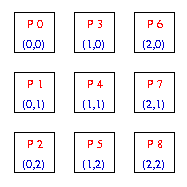
\includegraphics{topo}


\subsection{Cluster Information }

The following functions can be used to obtain information like number
of nodes that the program is running on, node ID of the process, and
other cluster information as discussed below:

The function

\textcolor{blue}{Fortran}~integer~function~\href{https://hpc.pnl.gov/globalarrays/api/f_op_api.html\#ga_cluster_nnodes}{ga\_{}cluster\_{}nnodes}()~

\textcolor{blue}{C}~~~~~~~int~\href{https://hpc.pnl.gov/globalarrays/api/c_op_api.html\#ga_cluster_nnodes}{GA\_{}Cluster\_{}nnodes}()~

\textcolor{blue}{C++}~~~~~int~GA::GAServices::clusterNnodes()

returns the total number of nodes that the program is running on.
On SMP architectures, this will be less than or equal to the total
number of processors.

The function

\textcolor{blue}{Fortran}~integer~function~\href{https://hpc.pnl.gov/globalarrays/api/f_op_api.html\#ga_cluster_nodeid}{ga\_{}cluster\_{}nodeid}()~

\textcolor{blue}{C}~~~~~~~int~\href{https://hpc.pnl.gov/globalarrays/api/c_op_api.html\#ga_cluster_nodeid}{GA\_{}Cluster\_{}nodeid}()~

\textcolor{blue}{C++}~~~~~int~GA::GAServices::clusterNodeid()

returns the node ID of the process. On SMP architectures with more
than one processor per node, several processes may return the same
node id.

The function

\textcolor{blue}{Fortran}~integer~function~\href{https://hpc.pnl.gov/globalarrays/api/f_op_api.html\#ga_cluster_nprocs}{ga\_{}cluster\_{}nprocs}(inode)

\textcolor{blue}{C}~~~~~~~int~\href{https://hpc.pnl.gov/globalarrays/api/c_op_api.html\#ga_cluster_nprocs}{GA\_{}Cluster\_{}nprocs}(int~inode)~

\textcolor{blue}{C++~~~~}~int~GA::GAServices::clusterNprocs(int~inode)

returns the number of processors available on node inode.

The function

\textcolor{blue}{Fortran}~integer~function~\href{https://hpc.pnl.gov/globalarrays/api/f_op_api.html\#ga_cluster_procid}{ga\_{}cluster\_{}procid}(inode,~iproc)~

\textcolor{blue}{C}~~~~~~~int~\href{https://hpc.pnl.gov/globalarrays/api/c_op_api.html\#ga_cluster_procid}{GA\_{}Cluster\_{}procid}(int~inode,~int~iproc)~

\textcolor{blue}{C++}~~~~~int~GA::GAServices::clusterProcid(int~inode,~int~iproc)

returns the processor id associated with node inode and the local
processor id iproc. If node inode has N processors, then the value
of iproc lies between 0 and N-1.

\textit{\underbar{Example:}} 2 nodes with 4 processors each. Say,
there are 7 processes created. Assume 4 processes on node 0 and 3
processes on node 1. In this case: number of nodes=2, node id is either
0 or 1 (for example, nodeid of process 2 is 0), number of processes
in node 0 is 4 and node 1 is 3. The global rank of each process is
shown in the figure and also the local rank (rank of the process within
the node.i.e., \texttt{cluster\_procid}) is shown in the parenthesis.

\begin{flushleft}
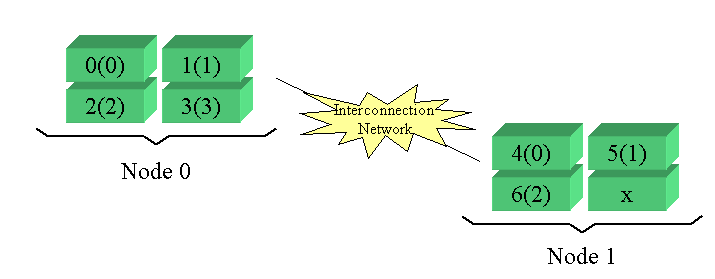
\includegraphics[width=4in]{cluster}
\par\end{flushleft}


\section{Memory Availability }

Even though the memory management does not have to be performed directly
by the user, Global Arrays provide functions to verify the memory
availability. Global Arrays provide the following information:
\begin{enumerate}
\item How much memory has been used by the allocated global arrays. 
\item How much memory is left for allocation of new the global arrays. 
\item Whether the memory in global arrays comes from the \href{https://hpc.pnl.gov/globalarrays/ma/MAapi.html}{Memory Allocator (MA)}. 
\item Is there any limitation for the memory usage by the Global Arrays.
\end{enumerate}
The function

\textcolor{blue}{Fortran~}integer~function~\href{https://hpc.pnl.gov/globalarrays/api/f_op_api.html\#ga_inquire_memory}{ga\_{}inquire\_{}memory}()~

\textcolor{blue}{C}~~~~~~~size\_t~\href{https://hpc.pnl.gov/globalarrays/api/c_op_api.html\#ga_inquire_memory}{GA\_{}Inquire\_{}memory}()~

\textcolor{blue}{C++~}~~~~size\_t~GA::GAServices::inquireMemory()

answers the first question. It returns the amount of memory (in bytes)
used in the allocated global arrays on the calling processor.

The function

\textcolor{blue}{Fortran}~integer~function~\href{https://hpc.pnl.gov/globalarrays/api/f_op_api.html\#ga_memory_avail}{ga\_{}memory\_{}avail}()~

\textcolor{blue}{C}~~~~~~~size\_t~\href{https://hpc.pnl.gov/globalarrays/api/c_op_api.html\#ga_memory_avail}{GA\_{}Memory\_{}avail}()~

\textcolor{blue}{C++}~~~~~size\_t~GA::GAServices::memoryAvailable()

answers the second question. It returns the amount of memory (in bytes)
left for allocation of new global arrays on the calling processor.

\href{https://hpc.pnl.gov/globalarrays/ma/MAapi.html}{Memory Allocator (MA)}
is a library of routines that comprises a dynamic memory allocator
for use by C, Fortran, or mixed-language applications. Fortran- 77
applications require such a library because the language does not
support dynamic memory allocation. C (and Fortran-90) applications
can benefit from using MA instead of the ordinary malloc() and free()
routines because of the extra features MA provides. The function

\textcolor{blue}{Fortran}~logical~function~\href{https://hpc.pnl.gov/globalarrays/api/f_op_api.html\#ga_uses_ma}{ga\_{}uses\_{}ma}()~

\textcolor{blue}{C}~~~~~~~int~\href{https://hpc.pnl.gov/globalarrays/api/c_op_api.html\#ga_uses_ma}{GA\_{}Uses\_{}ma}()~

\textcolor{blue}{C++}~~~~~int~GA::GAServices::usesMA()

tells whether the memory in Global Arrays comes from the Memory Allocator
(MA) or not.

The function

\textcolor{blue}{Fortran}~logical~function~\href{https://hpc.pnl.gov/globalarrays/api/f_op_api.html\#ga_memory_limited}{ga\_{}memory\_{}limited}()~

\textcolor{blue}{C}~~~~~~~int~\href{https://hpc.pnl.gov/globalarrays/api/c_op_api.html\#ga_memory_limited}{GA\_{}Memory\_{}limited}()~

\textcolor{blue}{C++}~~~~~int~GA::GAServices::memoryLimited()

Indicates if a limit is set on memory usage in Global Arrays on the
calling processor. 


\section{Message-Passing Wrappers to Reduce/Broadcast Operations }

Global Arrays provide convenient operations for broadcast/reduce regardless
of the message-passing library the process is running with.

The function

\textcolor{blue}{Fortran}~subroutine~\href{https://hpc.pnl.gov/globalarrays/api/f_op_api.html\#ga_brdcst}{ga\_{}brdcst}(type,~buf,~lenbuf,~root)~

\textcolor{blue}{C}~~~~~~~void~\href{https://hpc.pnl.gov/globalarrays/api/c_op_api.html\#ga_brdcst}{GA\_{}Brdcst}(void~{*}buf,~int~lenbuf,~int~root)~

\textcolor{blue}{C++}~~~~~void~GA::GAServices::brdcst(void~{*}buf,~int~lenbuf,~int~root)

broadcasts from process root to all other processes a message buffer
of length lenbuf.

The functions

\textcolor{blue}{Fortran}~subroutine~\href{https://hpc.pnl.gov/globalarrays/api/f_op_api.html\#ga_igop}{ga\_{}igop}(type,~x,~n,~op)~

~~~~~~~~subroutine~\href{https://hpc.pnl.gov/globalarrays/api/f_op_api.html\#ga_igop}{ga\_{}dgop}(type,~x,~n,~op)~

\textcolor{blue}{C}~~~~~~~void~\href{https://hpc.pnl.gov/globalarrays/api/c_op_api.html\#ga_igop}{GA\_{}Igop}(long~x{[}{]},~int~n,~char~{*}op)~

~~~~~~~~void~\href{https://hpc.pnl.gov/globalarrays/api/c_op_api.html\#ga_dgop}{GA\_{}Dgop}(double~x{[}{]},~int~n,~char~{*}op)~

\textcolor{blue}{C++}~~~~~void~GA::GAServices::igop(long~x{[}{]},~int~n,~char~{*}op)~

~~~~~~~~void~GA::GAServices::dgop(double~x{[}{]},~int~n,~char~{*}op)

'sum' elements of \emph{X(1:N)} (a vector present on each process)
across all nodes using the communicative operator \texttt{op}, The
result is broadcasted to all nodes. Supported operations include
\textbf{+,~{*},~max,~min,~absmax,~absmin}.
The integer version also includes the \texttt{\textbf{bitwise OR }}operation.

These operations unlike \texttt{ga\_sync}, do not include embedded
\texttt{ga\_gence} operations. 


\section{Others }

There are some other useful functions in Global Arrays. One group
is about inquiring the array attributes. Another group is about printing
the array or part of the array. 


\subsection{Inquire }

A global array is represented by a handle. Given a handle, one can
get the array information, such as the array name, memory used, array
data type, and array dimension information, with the help of the following
functions.

The functions

\textcolor{green}{n-D}~\textcolor{blue}{Fortran}~subroutine~\href{https://hpc.pnl.gov/globalarrays/api/f_op_api.html\#ga_inquire}{nga\_{}inquire}(g\_a,~type,~ndim,~dims)~

\textcolor{green}{2-D}~\textcolor{blue}{Fortran}~subroutine~\href{https://hpc.pnl.gov/globalarrays/api/f_op_api.html\#ga_inquire}{nga\_{}inquire}(g\_a,~type,~dim1,~dim2)~

\textcolor{blue}{C}~~~~~~~~~~~void~\href{https://hpc.pnl.gov/globalarrays/api/c_op_api.html\#ga_inquire}{NGA\_{}Inquire}(int~g\_a,~int~{*}type,~int~

~~~~~~~~~~~~~~~~~~~~{*}ndim,~int~dims{[}{]})~

\textcolor{blue}{C++}~~~~~~~~~void~GA::GlobalArray::inquire(int~{*}type,~int~

~~~~~~~~~~~~~~~~~~~~{*}ndim,~int~dims{[}{]})

return the data type of the array, and also the dimensions of the
array.

The function

\textcolor{blue}{Fortran}~subroutine~\href{https://hpc.pnl.gov/globalarrays/api/f_op_api.html\#ga_inquire_name}{ga\_{}inquire\_{}name}(g\_a,~array\_name)~

\textcolor{blue}{C}~~~~~~~char{*}~\href{https://hpc.pnl.gov/globalarrays/api/c_op_api.html\#ga_inquire_name}{GA\_{}Inquire\_{}name}(int~g\_a)~~

\textcolor{blue}{C++}~~~~~char{*}~GA::GlobalArray::inquireName()

finds out the name of the array.

One can also inquire the memory being used with \texttt{ga\_inquire\_memory}
(discussed above). 


\subsection{Print }

Global arrays provide functions to print
\begin{enumerate}
\item content of the global array 
\item content of a patch of global array 
\item the status of array operations 
\item a summary of allocated arrays
\end{enumerate}
The function

\textcolor{blue}{Fortran}~subroutine~\href{https://hpc.pnl.gov/globalarrays/api/f_op_api.html\#ga_print}{ga\_{}print}(g\_a)~

\textcolor{blue}{C}~~~~~~~void~\href{https://hpc.pnl.gov/globalarrays/api/c_op_api.html\#ga_print}{GA\_{}Print}(int~g\_a)~

\textcolor{blue}{C++}~~~~~void~GA::GlobalArray::print()

prints the entire array to the standard output. The output is formatted.

A utility function is provided to print data in the patch, which is

\textcolor{blue}{Fortran}~subroutine~\href{https://hpc.pnl.gov/globalarrays/api/f_op_api.html\#ga_print_patch}{nga\_{}print\_{}patch}(g\_a,~lo,~hi,~pretty)~

\textcolor{blue}{C}~~~~~~~void~\href{https://hpc.pnl.gov/globalarrays/api/c_op_api.html\#ga_print_patch}{NGA\_{}Print\_{}patch}(int~g\_a,~int~lo{[}{]},~

~~~~~~~~~~~~~~~~~~~int~hi{[}{]},~int~pretty)~

\textcolor{blue}{C++}~~~~~void~GA::GlobalArray::printPatch(int~lo{[}{]},~

~~~~~~~~~~~~~~~~~~~int~hi{[}{]},~int~pretty)

One can either specify a formatted output (set \texttt{pretty} to
one) where the output is formatted and rows/ columns are labeled,
or (set \texttt{pretty} to zero) just dump all the elements of this
patch to the standard output without any formatting.

The function

\textcolor{blue}{Fortran}~subroutine~\href{https://hpc.pnl.gov/globalarrays/api/f_op_api.html\#ga_print_stats}{ga\_{}print\_{}stats}()~

\textcolor{blue}{C}~~~~~~~void~\href{https://hpc.pnl.gov/globalarrays/api/c_op_api.html\#ga_print_stats}{GA\_{}Print\_{}stats}()~

\textcolor{blue}{C++}~~~~~void~GA::GAServices::printStats()

prints the global statistics information about array operations for
the calling process, including
\begin{itemize}
\item number of calls to the GA create/duplicate, destroy, get, put, scatter,
gather, and read\_and\_inc operations 
\item total amount of data moved in the GA primitive operations 
\item amount of data moved in GA primitive operations to logically remote
locations 
\item maximum memory consumption in global arrays, the \textquotedbl{}high-water
mark\textquotedbl{}
\end{itemize}
The function

\textcolor{blue}{Fortran}~subroutine~\href{https://hpc.pnl.gov/globalarrays/api/f_op_api.html\#ga_print_distribution}{ga\_{}print\_{}distribution}(g\_a)~

\textcolor{blue}{C~}~~~~~~void~\href{https://hpc.pnl.gov/globalarrays/api/c_op_api.html\#ga_print_distribution}{GA\_{}Print\_{}distribution}(int~g\_a)

\textcolor{blue}{C}~~~~~~~void~GA::GlobalArray::printDistribution()

prints the global array distribution. It shows mapping array data
to the processes.

The function

\textcolor{blue}{Fortran}~subroutine~\href{https://hpc.pnl.gov/globalarrays/api/f_op_api.html\#ga_summarize}{ga\_{}summarize}(verbose)~

\textcolor{blue}{C~}~~~~~~void~\href{https://hpc.pnl.gov/globalarrays/api/c_op_api.html\#ga_summarize}{GA\_{}Summarize}(int~verbose)~

\textcolor{blue}{C++}~~~~~void~GA::GAServices::summarize(int~verbose)

prints info about allocated arrays. verbose can be either one or zero. 


\subsection{Miscellaneous }

The function

\textcolor{blue}{Fortran}~subroutine~\href{https://hpc.pnl.gov/globalarrays/api/f_op_api.html\#ga_check_handle}{ga\_{}check\_{}handle}(g\_a,~string)~

\textcolor{blue}{C~~}~~~~~void~\href{https://hpc.pnl.gov/globalarrays/api/c_op_api.html\#ga_check_handle}{GA\_{}Check\_{}handle}(int~g\_a,~char~{*}string)

\textcolor{blue}{C++}~~~~~void~GA::GlobalArray::checkHandle(char~{*}string)

checks if the global array handle \texttt{g\_a} represents a valid
array. The \texttt{string} is the message to be printed when the handle
is invalid.
